\documentclass[svgnames,11pt]{beamer}
\input{/home/tof/Documents/Cozy/latex-include/preambule_commun.tex}
\input{/home/tof/Documents/Cozy/latex-include/preambule_beamer.tex}
%\usepackage{pgfpages} \setbeameroption{show notes on second screen=left}
\author[]{Christophe Viroulaud}
\title{Tests unitaires}
\date{\framebox{\textbf{Algo 16}}}
%\logo{}
\institute{Terminale - NSI}
\usetikzlibrary{shapes}
\begin{document}
\begin{frame}
    \titlepage
\end{frame}
\begin{frame}
    \frametitle{}

    Une tâche importante d'un programmeur est de garantir le bon comportement de son code, dans tous les cas de figures.

    \note{c'est une tâche difficile et chronophage}
\end{frame}
\begin{frame}
    \frametitle{}

    \begin{framed}
        \centering Comment mettre en place des tests unitaires?
    \end{framed}

\end{frame}
\section{Nécessité de tester}
\begin{frame}[fragile]
    \frametitle{Nécessité de tester}

    \begin{center}
        \begin{lstlisting}[language=Python , basicstyle=\ttfamily\small, xleftmargin=2em, xrightmargin=2em]
def images(deb, fin: int) -> list:
    """
    calcule les images d'une fonction
    """
    tab = []
    for i in range(deb, fin):
        tab.append(f(i))
    return tab

def f(x: int) -> float:
    return 1/x
\end{lstlisting}
        \begin{lstlisting}[language=Python , basicstyle=\ttfamily\small, xleftmargin=2em, xrightmargin=2em]
>>> images(1, 5)
[1.0, 0.5, 0.3333333333333333, 0.25]
>>> images(0, 5)
ZeroDivisionError: division by zero
\end{lstlisting}
    \end{center}

\end{frame}
\begin{frame}
    \begin{itemize}
        \item Un projet est composé de nombreux modules, eux-mêmes découpés en plusieurs fonctions.
        \item Une fonction \textbf{\texttt{f1}} peut utiliser le résultat renvoyé par une fonction \textbf{\texttt{f2}} qui utilise le résultat de \textbf{\texttt{f3}}\dots
    \end{itemize}

    \begin{aretenir}[]
        Chaque fonction doit être testée individuellement, pour chaque cas de figure.
    \end{aretenir}

\end{frame}
\section{Repérer les cas limites}
\begin{frame}[fragile]
    \frametitle{Repérer les cas limites}
    \begin{aretenir}[Observation]
        La fonction \textbf{\texttt{f}} impose des contraintes mathématiques.
    \end{aretenir}

    \begin{center}
        \begin{lstlisting}[language=Python , basicstyle=\ttfamily\small, xleftmargin=2em, xrightmargin=2em]
def images(deb, fin: int) -> list:
    """
    calcule les images d'une fonction
    """
    tab = []
    for i in range(deb, fin):
        tab.append(f(i))
    return tab

def f(x: int) -> float:
    return 1/x
\end{lstlisting}
    \end{center}

\end{frame}
\begin{frame}[fragile]
    \frametitle{}

    \begin{center}
        \begin{lstlisting}[language=Python , basicstyle=\ttfamily\small, xleftmargin=2em, xrightmargin=2em]
def f(x: int) -> float:
    assert x != 0, "pas de division par zéro"
    return 1/x
\end{lstlisting}
        \captionof{code}{Mettre en place des \textbf{assertions}}
    \end{center}

\end{frame}
\begin{frame}[fragile]
    \frametitle{}

    \begin{center}
        \begin{lstlisting}[language=Python , basicstyle=\ttfamily\small, xleftmargin=1em, xrightmargin=0em]
def f(x: int) -> float:
    if x == 0:
        raise Exception("pas de division par 0")
    return 1/x
\end{lstlisting}
        \captionof{code}{Lever une \textbf{exception} personnalisée}
    \end{center}
    \begin{aretenir}[]
        Cette notion est hors-programme en Terminale.
    \end{aretenir}
\end{frame}
\section{Garantir le bon comportement}
\subsection{Mise en évidence}
\begin{frame}
    \frametitle{Garantir le bon comportement - Mise en évidence}

    \begin{aretenir}[]
        Même sans erreur mathématique, une fonction peut ne pas renvoyer le résultat attendu.
    \end{aretenir}
\end{frame}

\begin{frame}[fragile]
    \begin{activite}
        La fonction \textbf{\texttt{est\_complet}} doit renvoyer \textbf{\texttt{True}} si la matrice d'adjacence représente un graphe complet.
        \begin{center}
            \begin{lstlisting}[language=Python , basicstyle=\ttfamily\small, xleftmargin=0.2em, xrightmargin=-3em]
def est_complet(mat: list) -> bool:
    """
    vérifie si chaque sommet est relié à tous
    les autres (sauf lui même)
    """
    for ligne in range(len(mat)):
        for col in range(len(mat)):
            if ligne != col and mat[ligne][col] == 0:
                return False
    return True
\end{lstlisting}
        \end{center}
        Proposer un cas de figure où la fonction n'a pas le bon comportement.
    \end{activite}
\end{frame}
\begin{frame}[fragile]
    \frametitle{Correction}

    \begin{center}
        \begin{lstlisting}[language=Python , basicstyle=\ttfamily\small, xleftmargin=2em, xrightmargin=2em]
mat = [ [1, 1, 1, 1, 1],
        [1, 0, 1, 1, 1],
        [1, 1, 0, 1, 1],
        [1, 1, 1, 0, 1],
        [1, 1, 1, 1, 0]]
\end{lstlisting}
        \captionof{code}{La fonction renvoie \textbf{\texttt{True}} avec cette matrice.}
        \label{CODE}
    \end{center}

\end{frame}
\begin{frame}[fragile]
    \frametitle{}
    \begin{center}
        \begin{lstlisting}[language=Python , basicstyle=\ttfamily\small, xleftmargin=0.2em, xrightmargin=-4em]
def est_complet(mat: list) -> bool:
    """
    vérifie si chaque sommet est relié à tous
    les autres (sauf lui même)
    """
    for ligne in range(ordre(mat)):
        for col in range(ordre(mat)):
            if (ligne != col and mat[ligne][col] == 0) or \
                    (ligne == col and mat[ligne][col] == 1):
                return False
    return True
\end{lstlisting}
        \captionof{code}{La fonction correcte}
        \label{CODE}
    \end{center}


\end{frame}
\subsection{Automatiser les tests}
\begin{frame}
    \frametitle{Automatiser les tests}

    \begin{aretenir}[]
        L'objectif de la mise en place des tests unitaires est de proposer une structure qui garantira le bon comportement de chaque fonction tout au long de l'évolution du projet.
    \end{aretenir}

\end{frame}
\begin{frame}
    \frametitle{}
    Les tests doivent être:
    \begin{itemize}
        \item exhaustifs (possible?),
        \item évolutifs en fonction des modifications du projet,
        \item exécutables de manière automatisée.
    \end{itemize}
    \note[item]{tâche longue et qui peut paraitre inutile(on ne produit pas de code qui fait avancer le projet)}
    \note[item]{rôle souvent alloué à une équipe entière (dans gros projet)}
\end{frame}
\begin{frame}[fragile]
    \frametitle{}

    La bibliothèque Python \textbf{\texttt{unittest}} permet de réaliser des tests unitaires. La stratégie consiste à créer une classe qui hérite de \textbf{\texttt{unittest.TestCase}} puis d'écrire une méthode pour chaque fonction à tester.

    \begin{center}
        \begin{lstlisting}[language=Python , basicstyle=\ttfamily\small, xleftmargin=2em, xrightmargin=2em]
import unittest
from mathematiques import f # fonction inverse

class Tests(unittest.TestCase):

    def test_inverse(self):
        self.assertTrue(f(1.) == 1.)
        self.assertTrue(f(-1) == -1.)


if __name__=="__main__":
    unittest.main()
\end{lstlisting}
    \end{center}
\end{frame}
\begin{frame}[fragile]
    \frametitle{}
    \begin{lstlisting}[language=Python , basicstyle=\ttfamily\small, xleftmargin=1em, xrightmargin=0em]
import unittest
from mathematiques import f # fonction inverse

class Tests(unittest.TestCase):

    def test_inverse(self):
        self.assertTrue(f(1.) == 1.)
        self.assertTrue(f(-1) == -1.)

if __name__=="__main__":
    unittest.main()
\end{lstlisting}
    \begin{activite}
        \begin{enumerate}
            \item Créer un fichier \textbf{\texttt{mes\_tests.py}}
            \item Écrire le code précédent (adapter le nom du fichier).
        \end{enumerate}
    \end{activite}


\end{frame}
\begin{frame}[fragile]
    \frametitle{}

    \begin{activite}
        \begin{center}
            \begin{lstlisting}[language=Python , basicstyle=\ttfamily\small, xleftmargin=.5em, xrightmargin=0em]
def test_inverse_erreur(self):
    # vérifie que la valeur 0 provoque une erreur
    with self.assertRaises(ZeroDivisionError):
        f(0)
\end{lstlisting}
            \captionof{code}{Tester une erreur}
            \label{CODE}
        \end{center}
        Ajouter la méthode précédente.
    \end{activite}

\end{frame}
\begin{frame}
    \frametitle{}

    Il existe plusieurs assertions testables:
    \begin{center}
        \begin{tabular}{|*{2}{c|}}
            \hline
            Méthode                             & Vérification             \\
            \hline
            \textbf{\texttt{assertEqual(a, b)}} & \textbf{\texttt{a == b}} \\
            \hline
            \textbf{\texttt{assertIs(a, b)}}    & \textbf{\texttt{a is b}} \\
            \hline
            \textbf{\texttt{assertIn(a, b)}}    & \textbf{\texttt{a in b}} \\
            \hline
        \end{tabular}
    \end{center}

\end{frame}
\begin{frame}[fragile]
    \frametitle{}

    Il est possible de définir un environnement de test pour se rapprocher des conditions d'utilisation.
    \begin{center}
        \begin{lstlisting}[language=Python , basicstyle=\ttfamily\small, xleftmargin=2em, xrightmargin=2em]
class Tests(unittest.TestCase):

    def setUp(self):
        # on définit des attributs...
        self.val = 1

    def test_inverse(self):
        # ...utilisables dans les tests
        self.assertTrue(f(self.val) == 1.)
\end{lstlisting}
    \end{center}

\end{frame}

\begin{frame}[fragile]
\begin{activite}
Proposer un jeu de tests pour valider la fonction \textbf{\texttt{est\_complet}}.
\end{activite}
    \begin{lstlisting}[language=Python , basicstyle=\ttfamily\small, xleftmargin=0.2em, xrightmargin=-4em]
def est_complet(mat: list) -> bool:
    """
    vérifie si chaque sommet est relié à tous
    les autres (sauf lui même)
    """
    for ligne in range(len(mat)):
        for col in range(len(mat)):
            if (ligne != col and mat[ligne][col] == 0) or \
                    (ligne == col and mat[ligne][col] == 1):
                return False
    return True
\end{lstlisting}

\end{frame}
\begin{frame}[fragile]
    \frametitle{Correction}

\begin{lstlisting}[language=Python , basicstyle=\ttfamily\small, xleftmargin=0.2em, xrightmargin=0em]
class Tests(unittest.TestCase):

    def setUp(self):
        # solution non exhaustive
        self.mat_ok = [[0, 1, 1, 1, 1],
                       [1, 0, 1, 1, 1],
                       [1, 1, 0, 1, 1],
                       [1, 1, 1, 0, 1],
                       [1, 1, 1, 1, 0]]
        self.mat_no = [[1, 1, 1, 1, 1],
                       [1, 0, 1, 1, 1],
                       [1, 1, 0, 1, 1],
                       [1, 1, 1, 0, 1],
                       [1, 1, 1, 1, 0]]

    def test_complet(self):
        self.assertTrue(est_complet(self.mat_ok))
        self.assertFalse(est_complet(self.mat_no))
\end{lstlisting}

\end{frame}
\begin{frame}
    \frametitle{}

    \begin{aretenir}[]
    Pour prendre en compte tous les cas de figures, le nombre de tests peut être important.
    \end{aretenir}
\note{cas matrice vide?}
\end{frame}
\subsection{Tester de manière exhaustive}
\begin{frame}[fragile]
    \frametitle{Tester de manière exhaustive}

    \begin{aretenir}[]
        Pour tester un code il faut prendre en compte tous les cas de figures.
    \end{aretenir}
\begin{center}
\begin{lstlisting}[language=Python , basicstyle=\ttfamily\small, xleftmargin=2em, xrightmargin=2em]
def ma_fonction(a: int, b: int) -> tuple:
    if a != 0:
        b = 5 - a
    else:
        b = b - a
    if b > 3:
        b = b//a
    else:
        b = 0
    return (a, b)
\end{lstlisting}
\end{center}

\end{frame}

\begin{frame}
    \frametitle{}

    \begin{center}
        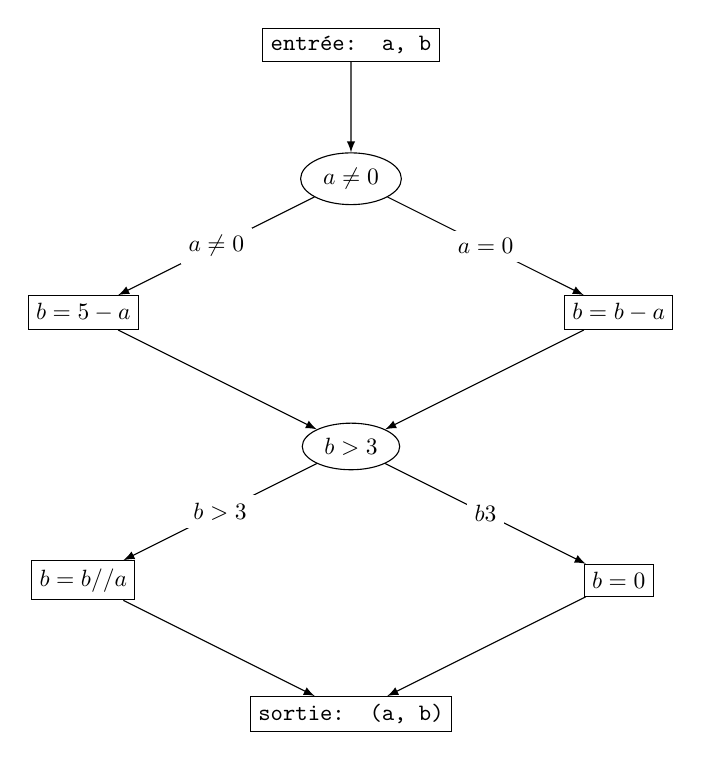
\begin{tikzpicture}[scale=0.85, transform shape]
            \node[draw] (0)at(0,4){\textbf{\texttt{entrée: a, b}}};
            \node[draw,ellipse] (1)at(0,2){\textbf{\texttt{$a\neq0$}}};
            \node[draw] (2)at(-4,0){\textbf{\texttt{$b=5-a$}}};
            \node[draw] (3)at(4,0){\textbf{\texttt{$b=b-a$}}};
            \node[draw,ellipse] (4)at(0,-2){\textbf{\texttt{$b>3$}}};
            \node[draw] (5)at(-4,-4){\textbf{\texttt{$b=b//a$}}};
            \node[draw] (6)at(4,-4){\textbf{\texttt{$b=0$}}};
            \node[draw] (7)at(0,-6){\textbf{\texttt{sortie: (a, b)}}};
            \draw[->,>=latex] (0)--(1);
            \draw[->,>=latex] (1)--(2) node[midway, fill=white] {$a\neq0$};
            \draw[->,>=latex] (1)--(3) node[midway, fill=white] {$a=0$};
            \draw[->,>=latex] (2)--(4);
            \draw[->,>=latex] (3)--(4);
            \draw[->,>=latex] (4)--(5) node[midway, fill=white] {$b>3$};
            \draw[->,>=latex] (4)--(6) node[midway, fill=white] {$b\leqslant 3$};
            \draw[->,>=latex] (5)--(7);
            \draw[->,>=latex] (6)--(7);

        \end{tikzpicture}
    \end{center}

\end{frame}
\begin{frame}
    \frametitle{}

    \begin{center}
        Pour tester \textbf{\texttt{ma\_fonction}} il faut choisir plusieurs couples de valeurs \textbf{\texttt{a, b}}.
    \end{center}

\end{frame}
\begin{frame}[fragile]
    \frametitle{}

    \begin{center}
        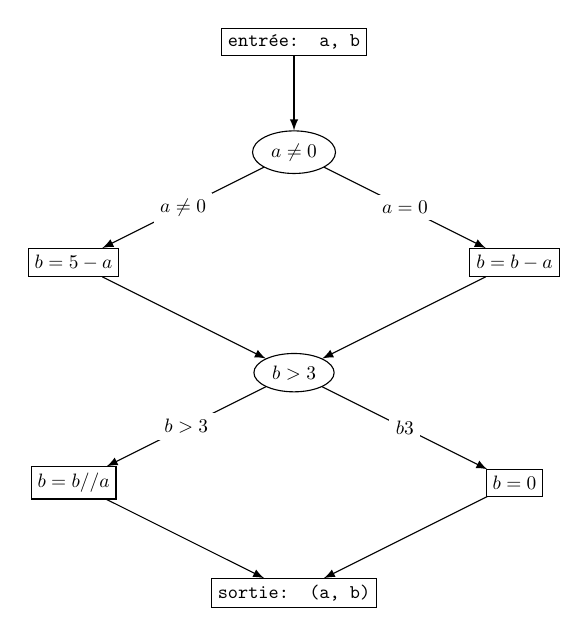
\begin{tikzpicture}[scale=0.7, transform shape]
            \node[draw] (0)at(0,4){\textbf{\texttt{entrée: a, b}}};
            \node[draw,ellipse] (1)at(0,2){\textbf{\texttt{$a\neq0$}}};
            \node[draw] (2)at(-4,0){\textbf{\texttt{$b=5-a$}}};
            \node[draw] (3)at(4,0){\textbf{\texttt{$b=b-a$}}};
            \node[draw,ellipse] (4)at(0,-2){\textbf{\texttt{$b>3$}}};
            \node[draw] (5)at(-4,-4){\textbf{\texttt{$b=b//a$}}};
            \node[draw] (6)at(4,-4){\textbf{\texttt{$b=0$}}};
            \node[draw] (7)at(0,-6){\textbf{\texttt{sortie: (a, b)}}};
            \draw[->,>=latex] (0)--(1);
            \draw[->,>=latex] (1)--(2) node[midway, fill=white] {$a\neq0$};
            \draw[->,>=latex] (1)--(3) node[midway, fill=white] {$a=0$};
            \draw[->,>=latex] (2)--(4);
            \draw[->,>=latex] (3)--(4);
            \draw[->,>=latex] (4)--(5) node[midway, fill=white] {$b>3$};
            \draw[->,>=latex] (4)--(6) node[midway, fill=white] {$b\leqslant 3$};
            \draw[->,>=latex] (5)--(7);
            \draw[->,>=latex] (6)--(7);

        \end{tikzpicture}
    \end{center}
\begin{lstlisting}[language=Python , basicstyle=\ttfamily\small, xleftmargin=2em, xrightmargin=2em]
ma_fonction(0, 3)
ma_fonction(1, 3)
\end{lstlisting}
\end{frame}
\begin{frame}
    \frametitle{}

    \begin{aretenir}[Observation]
    Toutes les arêtes ont été testées, cependant le risque de la division par zéro n'est pas montré.
    \end{aretenir}

\end{frame}
\begin{frame}[fragile]
    \frametitle{}

    \begin{center}
        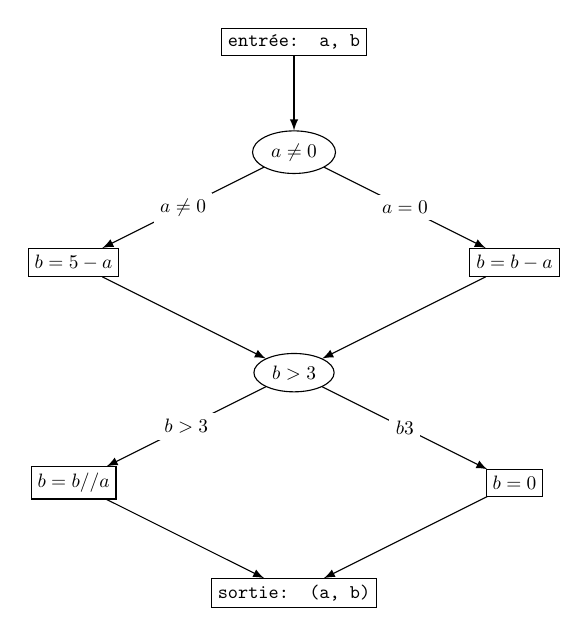
\begin{tikzpicture}[scale=0.7, transform shape]
            \node[draw] (0)at(0,4){\textbf{\texttt{entrée: a, b}}};
            \node[draw,ellipse] (1)at(0,2){\textbf{\texttt{$a\neq0$}}};
            \node[draw] (2)at(-4,0){\textbf{\texttt{$b=5-a$}}};
            \node[draw] (3)at(4,0){\textbf{\texttt{$b=b-a$}}};
            \node[draw,ellipse] (4)at(0,-2){\textbf{\texttt{$b>3$}}};
            \node[draw] (5)at(-4,-4){\textbf{\texttt{$b=b//a$}}};
            \node[draw] (6)at(4,-4){\textbf{\texttt{$b=0$}}};
            \node[draw] (7)at(0,-6){\textbf{\texttt{sortie: (a, b)}}};
            \draw[->,>=latex] (0)--(1);
            \draw[->,>=latex] (1)--(2) node[midway, fill=white] {$a\neq0$};
            \draw[->,>=latex] (1)--(3) node[midway, fill=white] {$a=0$};
            \draw[->,>=latex] (2)--(4);
            \draw[->,>=latex] (3)--(4);
            \draw[->,>=latex] (4)--(5) node[midway, fill=white] {$b>3$};
            \draw[->,>=latex] (4)--(6) node[midway, fill=white] {$b\leqslant 3$};
            \draw[->,>=latex] (5)--(7);
            \draw[->,>=latex] (6)--(7);

        \end{tikzpicture}
    \end{center}
\begin{lstlisting}[language=Python , basicstyle=\ttfamily\small, xleftmargin=2em, xrightmargin=2em]
ma_fonction(0, 4)
ma_fonction(2, 1)
\end{lstlisting}
\end{frame}
\begin{frame}
    \frametitle{}

    \begin{aretenir}[Edsger Dijkstra]
    \emph{Program testing can be used to show the presence of bugs, but never to show their absence.}
    \end{aretenir}
\begin{aretenir}[Traduction]
\emph{Le test peut être utilisé pour démontrer la présence de problèmes, mais jamais pour démontrer leur absence.}
\end{aretenir}
\end{frame}
\end{document}